The application of a stimulus to the nervous system leads to changes 
determined by two main properties:
\begin{itemize}
    \item \textbf{Excitability:} the capability of a nerve cell to react 
to an incoming impulse.
    \item \textbf{Plasticity:} certain permanent functional 
transformations arise in systems of neurons as a result of appropriate 
stimuli or their combination (it describes the possibility of the brain to 
maintain a specific response over long time scales).
\end{itemize}
The communication between neurons occurs through action potentials, as 
shown in the following picture.
\begin{figure}[H]
    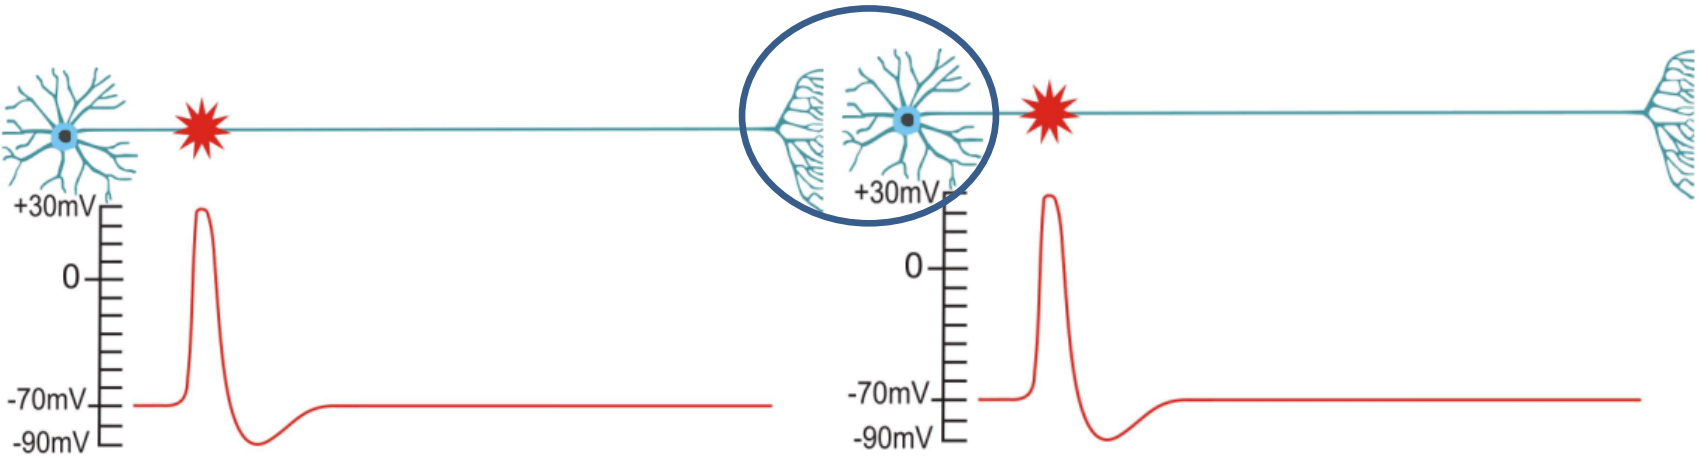
\includegraphics[scale=0.3]{1_1}
    \centering
\end{figure}
Measuring, analyzing, and processing brain signals is done for several 
reasons, but the three main ones are:
\begin{itemize}
    \item \textbf{Learn} more about the brain functioning.
    \item \textbf{Mimic} the brain functions in an artificial way to 
create new types of technologies - i.e. neuromorphic engineering.
    \item \textbf{Employ} brain signals for control and communication, as 
in the case of prosthetics.
\end{itemize}
This is what neuroengineering is actually about. It can be described as a 
tale of two loops: from one point of view, we have the development of new 
technologies from the knowledge of the brain, while from the other one, 
new technologies can be useful to treat the brain or the nervous system.\\

\paragraph{How to interact with the brain?}
Reading the neural code can be done through different levels of 
interaction of interfaces with the brain, and, depending on the scale
and depth, different signals can be obtained. 
\begin{itemize}
    \item \textbf{EEG:} electrodes placed on the scalp
    \item \textbf{Epidural and ECoG:} electrodes placed on the dura.
    \item \textbf{Intracortical:} electrodes placed in the cortex.
    \item \textbf{Depth:} electrodes placed in sub-cortical areas.
\end{itemize}
The neural code can either be read or written by exploiting several 
distinct techniques exhibiting different levels of:
\begin{align*}
    \begin{matrix}
        \textbf{Invasiveness}       &  & \textbf{Risk}                &  &
        \textbf{Spatial resolution} &  & \textbf{Temporal resolution}
    \end{matrix}
\end{align*}
The technology nowadays allows fair degrees of spatial and temporal 
resolutions, with
the main reading techniques being fMRI, PET, optical imaging, EEG, ECoG, 
MEA, single neuron, and others. Notice that also the number of reading 
sites is constantly increasing, due to the
exploitation of multiple electrode devices.
\begin{figure}[H]
    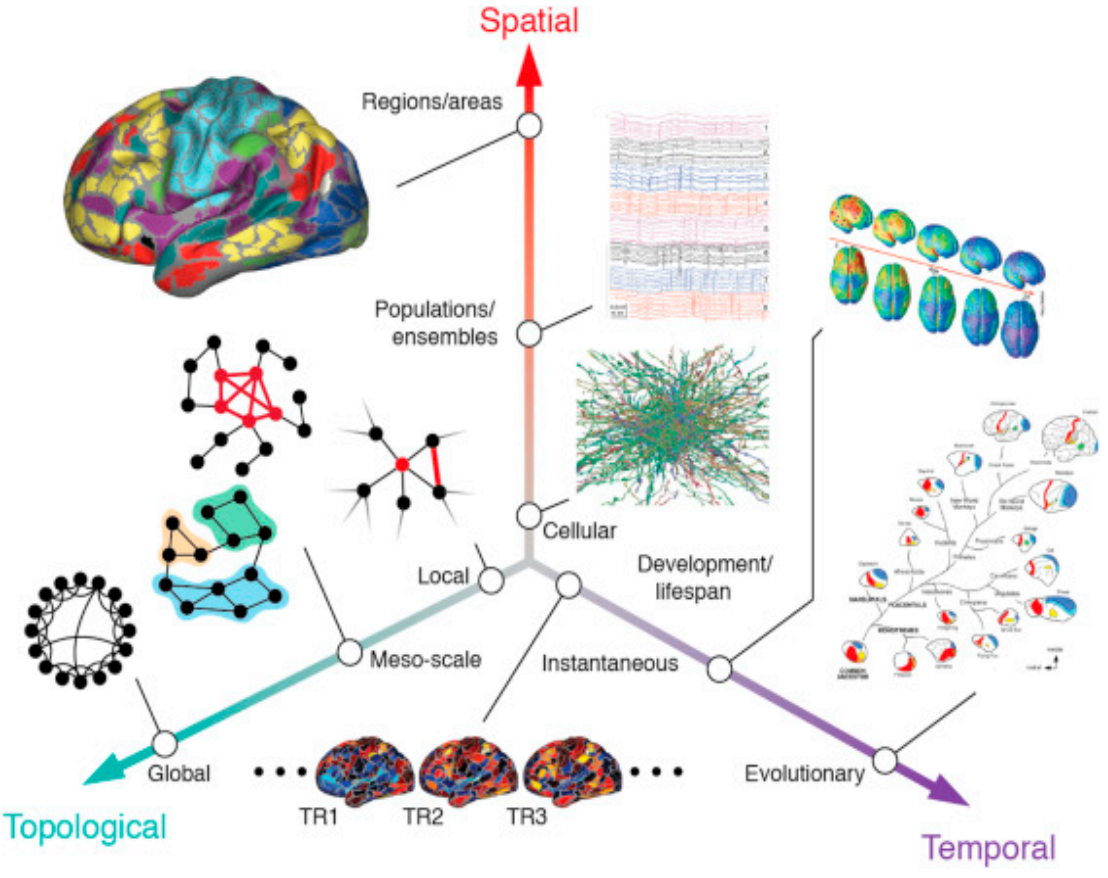
\includegraphics[scale=0.3]{1_2}
    \centering
\end{figure}
The multi-scale brain model presented above aims at showing the different 
levels at which the brain activity can be investigated, in terms of 
spatial, temporal, and topological scales.
Let's stress once more that the brain can be studied at different levels of 
complexity, which are somehow related to the risk due to the techniques 
involved to do so.
\begin{figure}[H]
    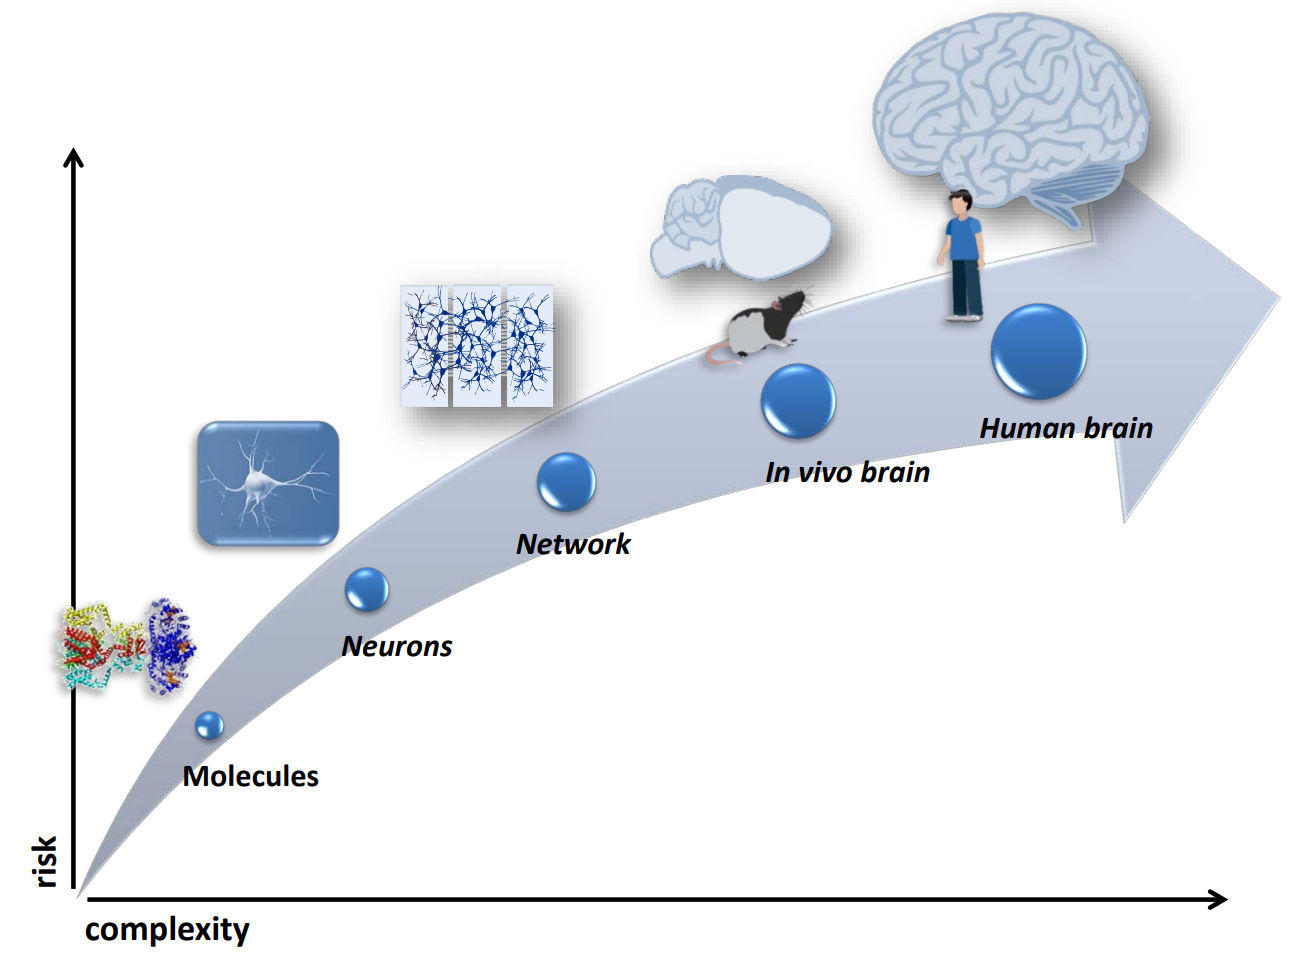
\includegraphics[scale=0.3]{1_3}
    \centering
\end{figure}
Notice that in general the functional unit of the brain is not a single 
neuron: it has soon been realized that the neurons, for the complexity of 
the complete structure, could not be studied only in isolation, but should 
also be analyzed in the different cell assemblies that they form.\\
There are many ways to study these structures, but in principle we can 
rely on two approaches: the \textit{in vitro} and \textit{in vivo} ones. 
Generally, this second family is more complex to employ, as it requires 
not to damage the brain of
the experiment subject.

\subsection{In Vitro Systems}
One of the principal technologies to study \textit{in vitro} networks is 
\textbf{MEAs (Micro Electrode Arrays)}, which are able to detect the 
activity of the network at several recording sites and for extended time 
periods.\\
They are composed by a complex integrated microelectrode system (with 
typically 60 sites), that leads to a multi-site long-term stimulation and 
recording.
However, an issue related to MEAs is the difficulty often encountered in 
analysing the recorded data
and interpreting the results in a meaningful way.\\
We can use these devices to record multiple types of signals, but the ones 
in which we are interested are mostly two:
\begin{itemize}
    \item \textbf{Local field potentials}, that can be acquired by 
recording the signal far from the neural network. They consist in the low 
frequency components (\(200/300\,Hz\)) accounting for several neurons as a sort 
of superposition of their effects.
    \item \textbf{Multi-unit activity}, which can be extracted by 
measuring a signal in the proximity of a neuron.  In general, a signal made 
of spikes is obtained by recording neural signals at high frequencies
(\(300\,Hz-3\,kHz\)), indicating the firing of a neuron. It is mostly related to the 
activity of one neuron but can also be influenced by the other ones 
nearby.
\end{itemize}

\textbf{Networks of neurons} represent an intermediate level of 
organization of the nervous system. 
In vitro neural networks are quite easy to obtain, and they are important, 
since they constitute a valuable experimental model for studying the 
collective electrophysiological and functional properties of the brain. In 
fact, the fundamental unit of the nervous system is not the single neuron,
rather the \textbf{cell assembly}.\\

Neurons dissociated from the original tissue can be cultured \textit{in vitro} from 
days up to months. During the \textit{in vitro} development, synapses start to be 
established and neurons begin to communicate among them, building a 2D 
network. Networks freely develop, without barriers, and the basic 
electrophysiological, biochemical and pharmacological properties are 
maintained similar to those of the \textit{in vivo} neurons.\\
These cultures are mostly obtained from animals, even if new technologies 
are being investigated and developed.\\
The process usually followed is:
\begin{itemize}
    \item \textbf{Pre-culture preparations:}
    \begin{itemize}
        \item Sterilize the culturing substrate (e.g. set of 
microelectrodes arrays).
        \item Pre-treat the insulation layer (silicon nitride) with 
adhesion factors (Poli-L/D-Lysine and Laminin) in order to improve the 
coupling between neurons and electrodes.
    \end{itemize}
    
    \item \textbf{Dissection:}
    \begin{itemize}
        \item Pregnant rats at the gestation day 18-19 are usually used. 
        \item The pups are removed and their cortex isolated.
    \end{itemize}
    
    \item \textbf{Dissociation:}
    \begin{itemize}
        \item Add trypsin.
        \item Mechanical dissociation by using a Pasteur pipette and cell 
count.
        \item Suspend the cells in neurobasal medium and place them on the 
pre-treated substrate (final concentration at about \(50.000\) cells/device).
    \end{itemize}
    
    \item \textbf{Maintenance of the culture:}
    \begin{itemize}
        \item Place the substrates in a humified incubator containing \(5\%\) 
of \(CO_2\) at \(37\,{}^{\circ}C\).
        \item Replace part of the old media with fresh media (neurobasal 
medium) each week.
    \end{itemize}
\end{itemize}

A few hours after dissociation, neurites start to elongate from the cell 
body and the first connections are established: neurons begin to 
communicate, and a new 2D network is created.
The main neurotrasmitters of the CNS - i.e. glutamate and GABA - are 
expressed after two weeks in culture.\\

\textit{In vitro} neural networks since they are extensively employed in research 
due to their fair level of organization and to the capability to easily
record their activity with arrays of electrodes. Nonetheless, some issues 
related to
\textit{in vitro} networks are the fact that they have no fidelity with 
respect to \textit{in vivo} neurons, starting from the fact that they 
generally arranged in 2D layers, instead of more complex three-dimensional 
networks.
However, new \textit{in vitro} approaches were recently developed, for example 3D 
structures like \textbf{brain organoids or spheroids}. This kind of models 
can be obtained also by human derived stem cells that can be 
differentiated into neurons. This allows to reduce the involvement of 
animals and customize the treatments for each patient.
\begin{figure}[H]
    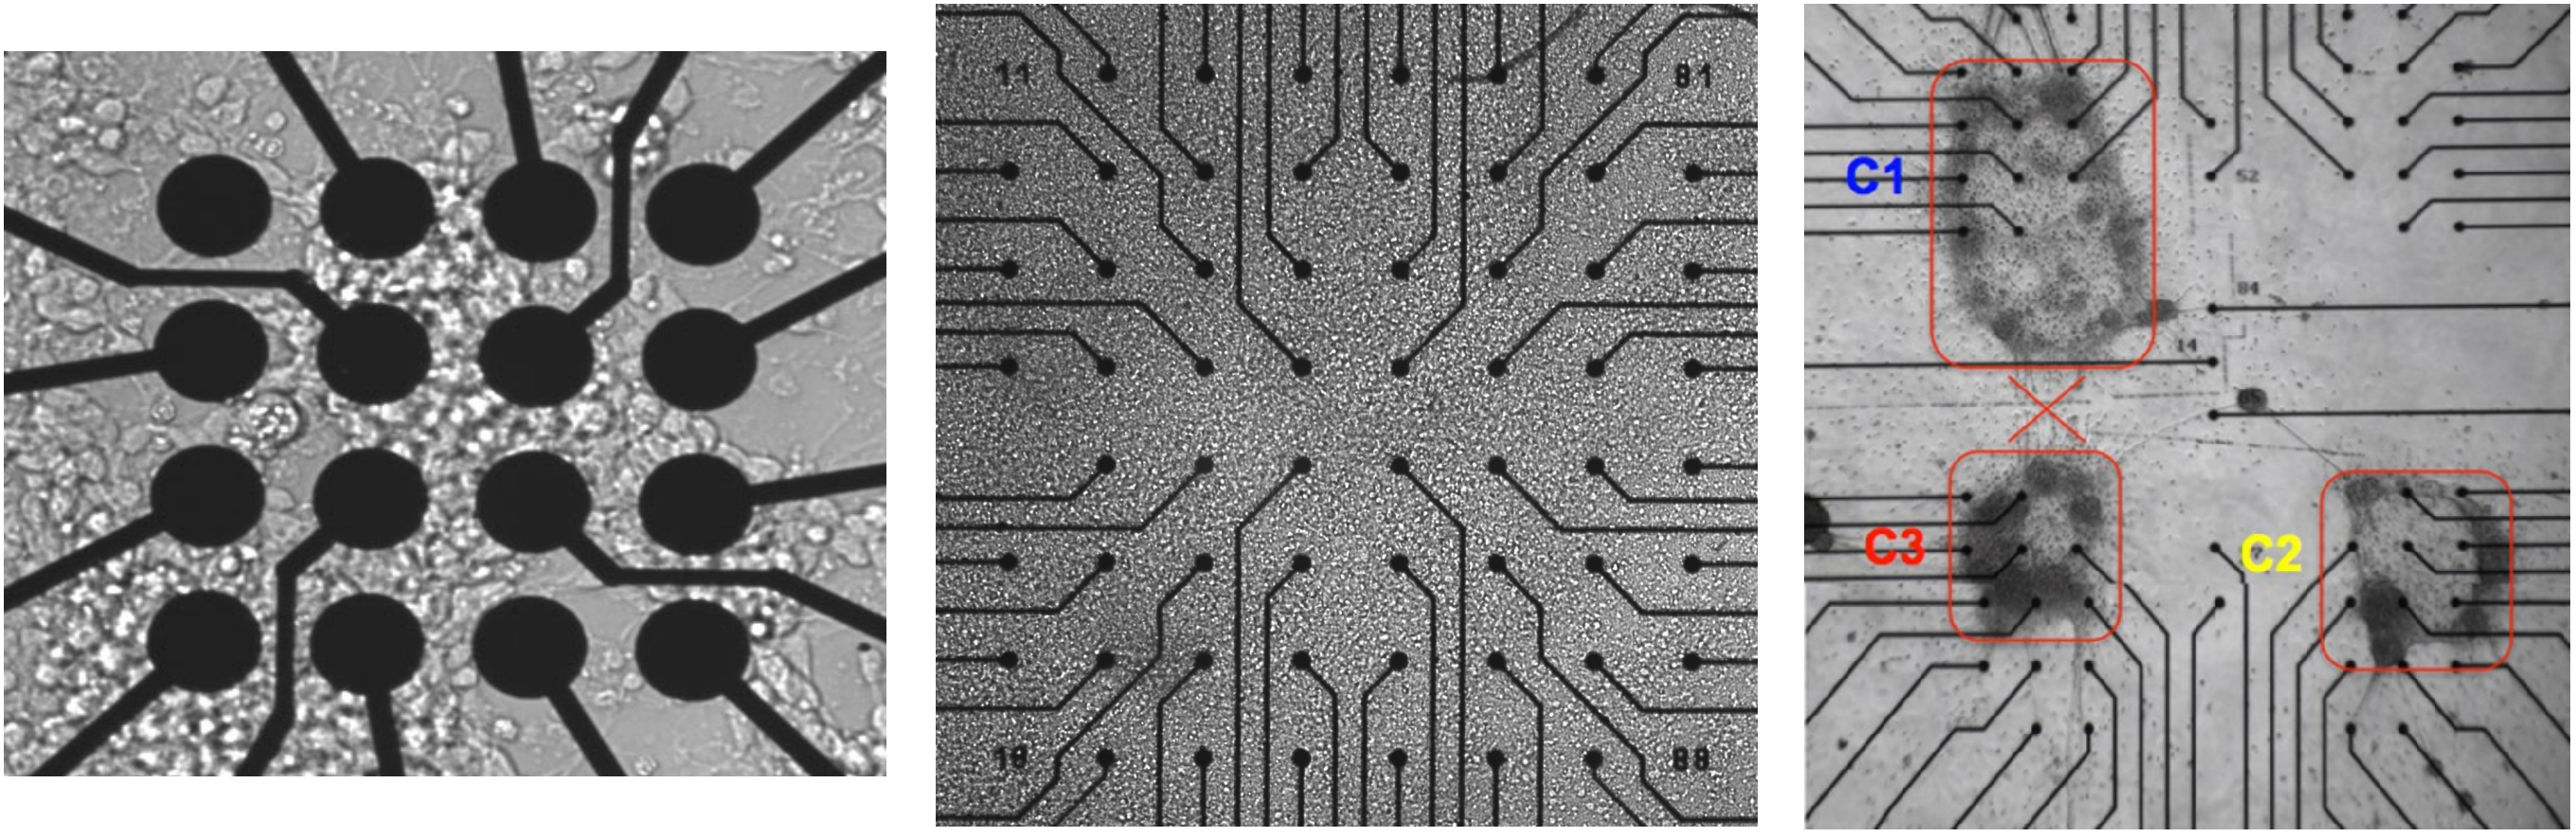
\includegraphics[scale=0.2]{1_4}
    \centering
\end{figure}
There is also another type of approach that we can use for \textit{in vitro} 
measurements, which is the one based on \textbf{brain slices}. In this 
model, brain slices maintain the same architecture of the brain from which 
they derive. The brain is glued onto the vibratome plate. The cut is 
performed in a very cold (\(0-2\,{}^{\circ}C\)) and oxygenated (\(95\%\) of \(O_2\)
and \(5\%\) of \(CO_2\)) physiological solution.
From this method we record mostly field potentials.\\

Another crucial concept is the one of brain modularity, as a matter of 
fact the brain is redundant and intrinsically modular, as it is composed of
local networks that are embedded into networks of networks.\\

\subsection{In Vivo Systems}
This kind of procedure is more complex: people must be trained to perform 
it and a specific environment is required. In this case, surgery is performed as
intracortical electrodes are to be implanted. The same experimental 
setup used for the \textit{in vitro} analysis can be also used for the \textit{in vivo} 
one.\\
\textbf{Calcium imaging} is another widely spread technique, which finds the 
variations of calcium in the tissue under the microscope. It can also be used 
for interconnected cells.

\subsection{From Raw Data to Point Process}
The most interesting process to consider is the detection of 
spikes, known as \textbf{Spike Detection}.
Spike trains are derived by filtering the raw signal recorded directly from the 
electrodes and by recognizing the spikes present in it. Notice that the 
crucial point is not the magnitude of a certain spike, rather its position 
on the time axis, indicating when it was fired.
\begin{figure}[H]
    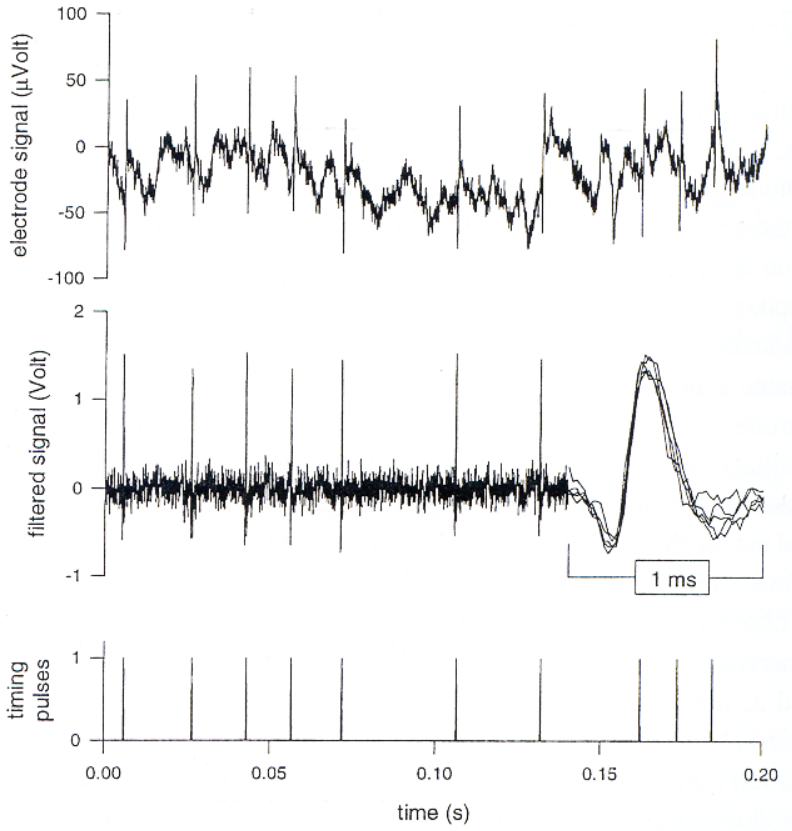
\includegraphics[scale=0.45]{1_5}
    \centering
\end{figure}
It is important to point out that the shape of a spike is highly 
influenced by the position of the measuring electrode w.r.t. the neuron 
that emitted it, enabling the researchers to recognize all the spikes 
emitted by the same source - i.e. a
particular neuron - and this is called Spike Sorting.\\
Simultaneous recording of multiple neurons offers new premises for 
investigating fundamental questions about brain functioning, provided that 
the challenging problem of analyzing multiple simultaneously recorded 
spike trains can be properly addressed.
There are some working assumptions that are usually done when studying 
spike trains:
\begin{itemize}
    \item There is an enormous wealth of information about the structure 
and function of the nervous system which can be derived from a careful study 
of the detailed timings of spike events. 
    \item The analysis of these signals can shed light on the mechanisms of 
spike production within the observed cell (on the pre-synaptic input) and 
the mechanisms by which the spike is transformed into a post-synaptic 
output.
    \item The observation of multiple units can reveal details regarding
interconnections and functional interactions.
    \item The neuronal processes at all levels involve a probabilistic element 
which should be adequately incorporated. 
\end{itemize}

Neural data present new analysis-related challenges as most standard signal 
processing techniques are designed primarily for continuous-valued data 
and not point processes. 
The main areas of research in this field are:
\begin{itemize}
    \item Identification and classification of spike events through Spike 
Detection and Spike Sorting.
    \item Novel techniques for measuring the degree of association between neural spike trains,
such as cross-correlograms, both in time and frequency domains. 
    \item Quantification of the neural response to a stimulus, by exploiting
techniques such as the PSTH.
\end{itemize}

Finally, let's highlight that the high number of electrodes employed in 
today's research implies a number of new challenges concerning data 
aquisition, storage, and analysis.\\
Since current techniques for spike train analysis are usually designed to 
analyze pairs of neurons, the challenge is to design methods 
that truly allow neuroscientists to perform multivariate analyses of 
multiple spike trains.
There are many benefits coming from the development of such methods:
\begin{itemize}
    \item Easier quantification of reliability and statistical 
significance of experimental findings.
    \item Easier correlation between neural ensemble dynamics and behavior 
for relevant biological stimuli.
    \item Possibility to design more complex experimental procedures to 
investigate more relevant and important scientific questions.
\end{itemize}

\subsection{Spike Trains}
A neuronal spike train is the sequence of nerve impulses or action 
potentials produced by a neuron and typically observed with either 
intracellular or extracellular microelectrodes over a relatively long 
period of time.\\
Spike train analysis differs from the classical electrophysiological methods 
as the raw data of interest are not precise voltage measurements but 
rather \textbf{precise measurements of times at which events occurred}. In 
fact, each spike is regarded as indistinguishable from the other ones produced by
the same neuron. Notice that the timing of a spike is given by the instant
of the maximum electrical potential excursion, which can be measured with
high degree of precision.\\
The most important properties of individual spike events are two:

\begin{itemize}
    \item \textbf{Indistinguishability:} spikes are characterized only by the
    time at which they occur, thus all spikes are assumed to have the same shape.
    \item \textbf{Instantaneity:} spikes are punctual events, with no duration.
    They can thus be described by pulses \(\delta\bigl(t-t_s\bigr)\).
\end{itemize}

In probability theory and statistics, a time series of discrete events, 
such as a spike train, is called a \textbf{point process}. More 
in-depth, a spike train is a one-dimensional stochastic point process characterized by a
certain degree of randomness and variability, where the only dimension of
interest is time.\\
Ensembles of spike trains from simultaneously recorded neurons are multi- 
dimensional point-process time series. These time series are both dynamic 
and stochastic. 

\begin{itemize}
    \item Dynamic means that their properties change through time
    \item Stochastic means that they change in a manner that can often be 
characterized by a probability model describing the likelihood of spikes 
at a given time. 
\end{itemize}

\paragraph{How to mathematically describe the spike train?} Given the
previously defined features of a spike, a spike train is immediately
defined as a sum of pulses:
\begin{equation*}
    ST(t) = \sum_{s=1}^N\delta(t-t_s)
\end{equation*}

For a network of \(M\) neurons, implying \(M\) simultaneously recorded
spike trains, the mathematical description is given by:
\begin{equation*}
    ST_j(t) = \sum_{s=1}^{N_j}\delta(t-t_s) \hspace{1 cm} j=1,\dots,M
\end{equation*}

\begin{figure}[h]
    \centering
    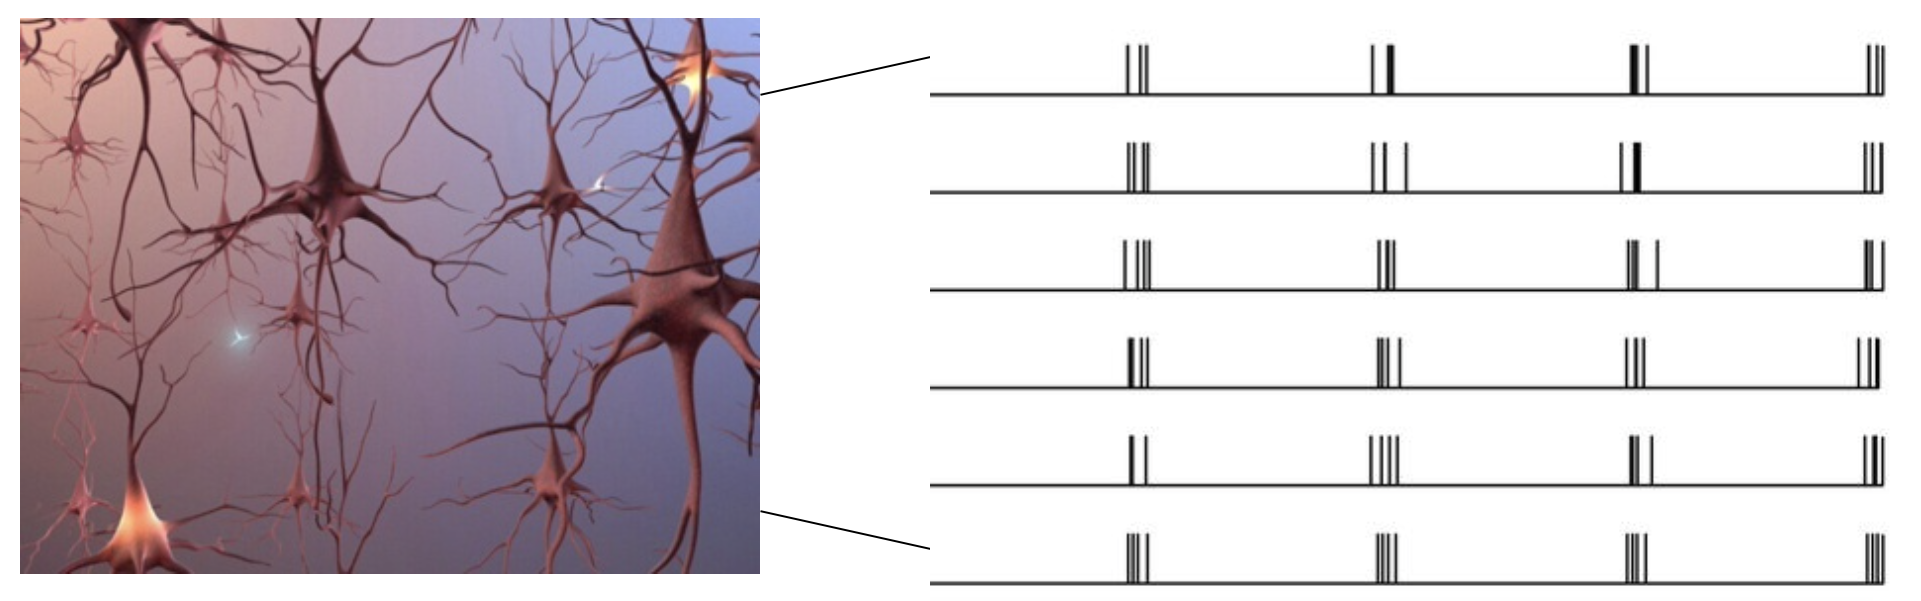
\includegraphics[scale=0.3]{1_6.png}
\end{figure}
\newpage
